
\documentclass[11pt,a4paper]{article}
\newcommand{\teamname}{VerteX}
\newcommand{\topicchoice}{Async Research Assistant}
\newcommand{\reportdate}{17 September 2026}
\newcommand{\repolink}{github.com/yagubbx/Research-Assistant}
\newcommand{\memberone}{Yaqub Xəlilli}
\newcommand{\membertwo}{Səbuhi Xamiyev}
\newcommand{\memberthree}{Aqil Əsgərov}

\usepackage[dvipsnames]{xcolor}
\definecolor{accent2}{HTML}{8B0000}
\definecolor{ph}{HTML}{6B7280}

\newcommand{\phh}[1]{\textcolor{ph}{\textit{#1}}}



\newcommand{\member}[2]{\textbf{#1} (#2)}  % name, GitHub handle



\newcommand{\coursecode}{AI-ENG-110}
\newcommand{\coursename}{Software Engineering}
\newcommand{\institution}{AI Academy, National AI Center}
\newcommand{\semester}{Spring 2026}

\usepackage[margin=2.2cm,headheight=15pt]{geometry}
\usepackage{fontspec}
\setmainfont{NotoSerif}[Path=../docs/fonts/,Extension=.ttf,UprightFont=*-Regular,BoldFont=*-Bold,ItalicFont=*-Italic,BoldItalicFont=*-BoldItalic]
\setsansfont{NotoSans}[Path=../docs/fonts/,Extension=.ttf,UprightFont=*-Regular,BoldFont=*-Bold,ItalicFont=*-Italic,BoldItalicFont=*-BoldItalic]
\setmonofont{texgyrecursor-regular.otf}

\usepackage[final,protrusion=true,expansion=false]{microtype}
\usepackage{amsmath,amssymb}
\usepackage{graphicx}
\usepackage{booktabs}
\usepackage{array}
\usepackage{tabularx}
\usepackage{ragged2e}
\usepackage{enumitem}
\usepackage[parfill]{parskip}
\usepackage{listings}
\usepackage[most]{tcolorbox}
\usepackage{titlesec}
\usepackage{fancyhdr}
\usepackage{lastpage}
\usepackage[hidelinks]{hyperref}

\emergencystretch=3em
\hbadness=10000
\hfuzz=2pt

\hypersetup{
  colorlinks=true,
  linkcolor=NavyBlue,
  urlcolor=NavyBlue,
  citecolor=NavyBlue,
  pdftitle={\coursecode\ Final Project Report},
  pdfauthor={\teamname}
}

\definecolor{accent}{HTML}{0B3D91}
\definecolor{soft}{HTML}{F2F4F8}
\definecolor{deliver}{HTML}{E8F0FE}
\definecolor{deliverframe}{HTML}{1A56DB}
\definecolor{probe}{HTML}{FFF8E1}
\definecolor{probeframe}{HTML}{B45309}

\titleformat{\section}
  {\Large\bfseries\color{accent}}{\thesection.}{0.6em}{}
\titleformat{\subsection}
  {\large\bfseries\color{accent}}{\thesubsection}{0.5em}{}

\newcommand{\ans}[1]{\rule[-2pt]{#1}{0.5pt}}
\let\ph\phh  % alias the early \phh as \ph for consistency with the body

\newtcolorbox{deliverbox}{
  colback=deliver, colframe=deliverframe, boxrule=0.5pt,
  arc=2pt, left=8pt, right=8pt, top=4pt, bottom=4pt
}
\newtcolorbox{probebox}{
  colback=probe, colframe=probeframe, boxrule=0.5pt,
  arc=2pt, left=8pt, right=8pt, top=4pt, bottom=4pt
}





\definecolor{codegreen}{rgb}{0,0.55,0}
\definecolor{codegray}{rgb}{0.4,0.4,0.4}
\definecolor{codepurple}{rgb}{0.55,0,0.78}
\definecolor{backcolour}{rgb}{0.97,0.97,0.97}

\lstdefinestyle{python}{
  language=Python,
  backgroundcolor=\color{backcolour},
  commentstyle=\color{codegreen},
  keywordstyle=\color{accent},
  numberstyle=\tiny\color{codegray},
  stringstyle=\color{codepurple},
  basicstyle=\ttfamily\footnotesize,
  breakatwhitespace=false,
  breaklines=true,
  keepspaces=true,
  numbers=left,
  numbersep=6pt,
  tabsize=2,
  frame=single,
  framerule=0.4pt,
  rulecolor=\color{black!30},
}

\pagestyle{fancy}
\fancyhf{}
\fancyhead[L]{\small\textit{\coursecode\ -- Final Report -- \teamname}}
\fancyhead[R]{\small\textit{\semester}}
\fancyfoot[L]{\small\textit{\institution}}
\fancyfoot[R]{\small Page \thepage\ of \pageref{LastPage}}
\renewcommand{\headrulewidth}{0.4pt}
\renewcommand{\footrulewidth}{0.4pt}

\usepackage{tikz}
\usetikzlibrary{arrows.meta,positioning}

\usepackage{xurl}
\begin{document}

\begin{center}
{\small\textsc{AI Academy, National AI Center}\\AI-ENG-110 -- Software Engineering -- Spring 2026}\\[1cm]
{\Large\bfseries\color{accent}Final Project Report}\\[0.4cm]
{\LARGE\bfseries Async Research Assistant}\\[0.5cm]
\rule{0.85\textwidth}{0.6pt}\\[0.5cm]
{\Large VerteX}\\[0.4cm]
Yaqub Xəlilli (\texttt{@yagubbx})\\
Səbuhi Xamiyev (\texttt{@KhamiyevSebuhi})\\
Aqil Əsgərov (\texttt{@agilasgarli-sys})\\[0.5cm]
\href{https://github.com/yagubbx/Research-Assistant}{github.com/yagubbx/Research-Assistant}\\[0.25cm]
Engineering verification: 17 September 2026\\
Release tag target: \texttt{v1.0-final}
\end{center}
\section*{Executive Summary}
This project implements the software-engineering layer for Topic 4 only. A question is validated, Wikipedia, arXiv and web search are queried concurrently, and the provided AI synthesizer produces an answer with numbered references. The supplied AI package and its 16 contract tests remain unchanged. The application adds typed configuration, independent deadlines, request retries, per-host pacing, a persistent TTL cache, structured diagnostics and a reproducible command-line interface. The final revision also adds local configuration diagnostics and separates optional provider SDKs from offline requirements.

The verification run passed 121 offline tests with 93.85\% application coverage. A five-question retrieval benchmark measured a median 2.412 seconds sequentially and 0.802 seconds concurrently, a 3.01-fold speedup. These are explicitly simulated HTTP timings with caches bypassed; they do not establish live provider latency or research quality.

The package includes source, tests, Docker configuration, this report, the defense slides and run artefacts. Docker build, offline CLI and container UI health checks passed; live Gemini research passed on Render with three sources and three references. PR 1 showed two successful checks and was merged into main (b56bd18). The operator reports Render now uses main; signatures and the final tag remain team actions. This report records engineering evidence rather than certifying a grade or submission status.

\clearpage
\section{Project Overview}
\subsection{Problem framing \& scope}
The user needs a concise answer whose sources can be inspected. The minimum contract is \texttt{python -m researcher ask "question"}. Optional flags select \texttt{wiki,arxiv,web}, bypass all cache reads and writes, emit JSON, or save the result. The \texttt{demo} command processes all five original questions. An explicit offline switch runs deterministic educational fixtures without credentials. Arbitrary questions are rejected in that mode, so canned evidence cannot be mistaken for general research.

\subsection{Provider choice and the AI module contract}
The delivered environment example selects Gemini gemini-3.1-flash-lite and keyless DuckDuckGo search. Alternative providers remain configurable. A live Render request completed in 23.21 seconds with three available sources and three references; its answer disclosed evidence limitations. This is one acceptance sample, not a provider quality or uptime guarantee. Application business logic never constructs provider SDK clients. All source fetching uses the three public \texttt{ai.fetch\_*} functions, and synthesis calls \texttt{ai.synthesize} in an isolated process.

\section{Architecture}
\subsection{Module map}

\begin{center}
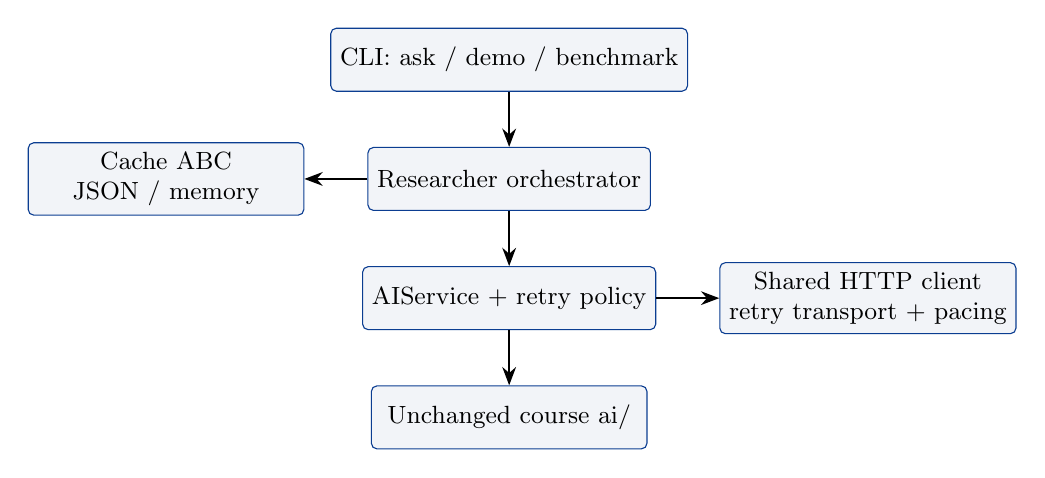
\begin{tikzpicture}[node distance=7mm,box/.style={draw=accent,rounded corners=2pt,fill=soft,align=center,minimum width=3.5cm,minimum height=8mm,font=\small},arr/.style={-Stealth,thick}]
\node[box] (cli) {CLI: ask / demo / benchmark};
\node[box,below=of cli] (core) {Researcher orchestrator};
\node[box,left=8mm of core] (cache) {Cache ABC\\JSON / memory};
\node[box,below=of core] (service) {AIService + retry policy};
\node[box,below=of service] (ai) {Unchanged course ai/};
\node[box,right=8mm of service] (http) {Shared HTTP client\\retry transport + pacing};
\draw[arr] (cli)--(core); \draw[arr] (core)--(cache);
\draw[arr] (core)--(service); \draw[arr] (service)--(ai); \draw[arr] (service)--(http);
\end{tikzpicture}
\end{center}

\subsection{OOP design \& data flow}
\texttt{Researcher} composes \texttt{AIService}, \texttt{Cache} and a semaphore. The abstract cache interface has independent JSON and memory implementations; its contract is tested against both. Stateful rate-limit bookkeeping belongs to \texttt{RateLimiter}. Pydantic models carry source outcomes, cached records and complete sessions across boundaries. Raw dictionaries are confined to serialization or external payload parsing. Pure validation functions own normalization and citation checks. CLI code renders results without duplicating business rules.

\clearpage
\section{Concurrency \& Performance}
\subsection{Why this concurrency model}
Retrieval is I/O-bound, so asynchronous HTTP allows the three independent sources to overlap. One shared \texttt{AsyncClient} serves a research request. The application uses \texttt{asyncio.gather(..., return\_exceptions=True)} as required. Each source receives its own total deadline, including semaphore wait, retries and rate pacing. Expected upstream failures become typed outcomes; unexpected programming errors propagate. A configurable semaphore defaults to three active source operations.

Synthesis is synchronous in the supplied package. A child process owns that call and communicates through JSON. A background thread waits for its pipes; the event loop remains responsive. On the synthesis deadline, the parent kills and reaps the worker, avoiding an uninterruptible SDK thread. The process startup cost is accepted to make the deadline meaningful.

\subsection{Sequential-vs-concurrent benchmark}
The benchmark processes the five provided questions on the same Windows host, using the same parsers and orchestrator. Each simulated source has 150 ms total delay; Wikipedia splits this into search and summary requests. Source caching is bypassed for reads and writes. Three repetitions alternate scheduling order to reduce order bias. Synthesis is excluded so the measured effect is retrieval overlap.
\begin{center}
\begin{tabular}{lrr}\toprule
Run & Sequential (s) & Parallel (s)\\\midrule
1 & 2.413 & 0.819\\
2 & 2.412 & 0.795\\
3 & 2.398 & 0.802\\
\midrule Median & 2.412 & 0.802\\
Speedup & 1.00 & 3.01\\\bottomrule
\end{tabular}
\end{center}
There were zero failed or empty simulated outcomes. The ideal overlap is roughly threefold; scheduling and parsing overhead explain the smaller observed ratio. The parallel retrieval bottleneck is the slowest source, especially Wikipedia's two ordered HTTP requests. In a full live run, synthesis and upstream rate limits may dominate. No live speedup is claimed.

\subsection{Live retrieval measurement}
Five topical queries against real Wikipedia/arXiv took 19.656 s sequential and 19.288 s parallel (1.02 times) in one repetition, with zero failed or empty outcomes. Both modes bypassed cache and retained provider pacing. This workload excludes web search and synthesis; its small gain illustrates network variation and rate-limit overhead. Raw per-query records and the reproducing script are shipped. This is separate from the synthetic three-source experiment.



\subsection{Rate limit \& politeness}
The per-host limiter behaves as a capacity-one bucket: normally one dispatch per second, with a three-second arXiv interval. It persists across questions within one orchestrator instance. HTTP 429 responses additionally honor \texttt{Retry-After}. Separate processes do not share budgets. Offline benchmarks disable pacing because they model network wait rather than upstream policy.

\clearpage
\section{Robustness \& Error Handling}
\subsection{Wrapping the AI module}
The default retry budget is three attempts, with 0.5 and 1.0 second delays. Transient transport failures, HTTP 429 and 5xx are retryable. Permanent HTTP authentication failures are returned without repeated calls. HTTP responses are fully read inside the retry boundary, including interrupted body streams. HTTP retries live below the course fetchers, so a Wikipedia summary request is protected even though the supplied code skips failed summaries. Exhausted HTTP failures are marked to prevent the outer AI wrapper multiplying the retry budget. Every source has a 20-second total deadline; each HTTP operation defaults to eight seconds. Synthesis has a separate 60-second deadline.

Errors cross the CLI boundary as concise messages and exit code 2. Cancellation returns 130. Runtime diagnostics use JSON-formatted logging on stderr; answers remain on stdout. Log messages record source, status, counts and duration, without raw exception messages, credentials or research payloads. This intentionally favors privacy over verbose payload logging.

\subsection{Failure-mode analysis: unavailable arXiv}
An injected \texttt{ProviderError} in arXiv verified the degradation path. Wikipedia and web evidence remained available; the synthesizer received only usable evidence. The final references included an explicit arXiv-unavailable note. The test also inserted a secret-like exception message and verified that it did not appear in the session JSON. A separate timeout test delayed arXiv beyond 50 ms and observed a timeout outcome while Wikipedia completed.

When every source fails or returns empty evidence, the application refuses synthesis. This avoids producing an answer with invented support. Invalid model output is regenerated within the retry/deadline budget, then rejected if still invalid: an empty answer, no valid citation, or a factual sentence without a citation produces a clear error. Structural validation cannot prove that the cited passage supports a claim; that remains a stated quality limitation.

\subsection{Input validation}
Questions must contain letters or numbers and cannot exceed the configured 2,000-character limit. Unknown source names are rejected before network work. ANSI escape sequences, HTML tags, invisible controls and bidirectional control characters are removed from displayed text. Only usable HTTP(S) source URLs and nonempty excerpts survive evidence validation. The citation validator removes invalid numeric markers from the answer itself and reconstructs references from the actual selected evidence, rather than trusting model-provided reference objects.

\clearpage
\section{Storage \& Caching}
\subsection{Schema}
Each JSON record contains a schema version, absolute expiry timestamp and a list of the provided \texttt{Source} models. A record is addressed by SHA-256 of namespace, source name and canonical query. Hashing prevents user input from becoming a filesystem path. Namespaces separate offline fixtures from live results and distinguish web provider and result-count settings. Evidence from a demo can therefore never satisfy a live cache lookup.

\begin{lstlisting}[style=python,numbers=none]
class CacheEntry(BaseModel):
    version: Literal[1] = 1
    expires_at: float
    sources: list[Source]
\end{lstlisting}

\subsection{Caching policy}
The default TTL is one hour and is configurable. Canonicalization applies Unicode normalization, case folding, whitespace collapsing and removal of a trailing question mark. It deliberately preserves meaningful punctuation: ``C++'' must not collide with ``C''. The cache key still includes the selected source. The CLI's \texttt{--no-cache} flag bypasses both reads and writes; benchmark runs always take this path.

A cache write goes to a unique temporary file and is atomically replaced into its destination. Readers see a complete old or new record. Concurrent writers for one query are last-writer-wins, which is acceptable for short-lived search excerpts. Corrupt, oversized, expired or inaccessible records become misses with a diagnostic. A failed cache write does not discard a successfully retrieved answer. Empty and failed retrievals are not persisted.

Filesystem access runs through a worker thread to avoid blocking source scheduling. The in-memory implementation exists for tests and embedded use. Filesystem JSON is suitable for this course CLI because it needs no database service and survives process restarts. PostgreSQL would add operational overhead without a demonstrated workload need.

\subsection{Trade-offs}
The cache is not a research history store: answers are recomputed and the CLI saves artefacts only when requested. TTL limits freshness at read time but does not immediately remove old files from disk. A long-running service should add eviction and a storage quota. Atomic replacement provides record integrity, not distributed locking or deduplication of concurrent misses. Independent CLI processes also maintain separate upstream rate budgets. These are explicit deployment limits, not hidden consistency guarantees.

\clearpage
\section{Testing}
\subsection{Strategy \& coverage}
The measured suite contains 121 passing tests, including all 16 unchanged course smoke tests. Coverage of the application package is 93.85\%, above the required 60\% gate. The course provider implementation is excluded from the application coverage denominator and separately exercised by its smoke tests. Raw coverage data is supplied in \texttt{artefacts/coverage.json}. Ruff passed after formatting; mypy reported no issues in 18 application files.

The suite uses fake AI responses, HTTPX mock transport and \texttt{respx}. A root fixture rejects real socket connections in the test process. Offline subprocess synthesis uses only the deterministic fixture LLM. CI additionally runs the container demo with networking disabled. The suite does not require API keys or a paid account.

\subsection{Notable tests}
\noindent\begin{tabularx}{\linewidth}{@{}p{3.3cm}>{\raggedright\arraybackslash}X@{}}\toprule
Area & Evidence and invariant\\\midrule
Orchestration & Happy path shares one client; arXiv failure and timeout preserve the answer; all-source failure prevents synthesis.\\
Concurrency & Instrumented tasks reach two simultaneous operations with a bound of two; delayed parallel retrieval beats the sequential baseline.\\
HTTP boundary & Mocked 429 and 503 responses recover; 401 is attempted once; connection failure exhausts its budget.\\
Cache & Both repositories pass miss, round-trip and expiry tests; disk tests cover corruption, namespace isolation and I/O failure.\\
Validation & Oversized and empty questions, source selection, unsafe URLs, dangling citations and uncited sentences are tested.\\
CLI and worker & Offline JSON, saved output, configuration errors, worker schema errors and hard synthesis timeout are exercised.\\\bottomrule
\end{tabularx}\par

\subsection{Interpretation}
Coverage measures executed lines, not scientific answer accuracy. The simulated fixtures are educational summaries, not scraped research evidence. The test results establish the application's control flow and resilience under the modeled failures. They do not establish a live provider's availability, output quality, current model names, or billing behavior. The timeout test is particularly useful because a normal success test would not detect a blocking SDK process left behind after cancellation.

\clearpage
\section{Deployment \& Reproducibility}
\subsection{Docker image}
The multi-stage Dockerfile builds dependency wheels and installs them into a Python 3.12 slim runtime. It runs as UID 10001, copies only the selected topic's code and sample data, and provides a writable cache directory. The default command processes all five offline questions. Secrets, local environments, cache contents and generated reports are excluded from the image context. Direct dependencies are version-pinned; transitive dependencies are resolved by pip and are not a byte-for-byte lock.

\begin{lstlisting}[style=python,language=bash,numbers=none]
docker build -t vertex-research .
docker run --rm --network none vertex-research
docker run --rm --env-file .env vertex-research \
  ask "What is photosynthesis?" --no-cache
\end{lstlisting}

The host Docker build, five-question offline run, doctor and Streamlit HTTP health checks passed; the saved acceptance log identifies the image. Its size is 338,510,564 bytes, so the 250 MB size bonus is not claimed. The included GitHub Actions workflow installs dependencies, lints, type-checks, runs tests with a coverage gate, builds the image and executes the offline container. The team supplied PR 1 evidence showing both checks successful before merge. Repository maintainers must require the quality job in branch protection.

\subsection{Configuration}
\texttt{Settings.from\_env} is the application configuration boundary. It loads a local \texttt{.env} without overriding shell values, validates numeric bounds and exposes typed fields. Provider names and models retain the course module's environment interface. The doctor command checks local credentials and SDK availability without network calls. Optional live SDKs are installed from the provider requirements file. The example file lists application limits, all provider key aliases used by the supplied package and optional inherited provider variables.

For a live run, configure one supported LLM key and a web-search key, or select a keyless web provider. Never commit the real \texttt{.env}. The command checks required credentials before retrieval. The README includes Windows and POSIX setup, examples, exit codes, Docker commands and commands to reproduce the benchmark.

\subsection{Problems resolved during integration}
Uncited model sentences triggered bounded regeneration rather than fabricated citations. Long question wording was reduced to a topic query for retrieval. Web search moved behind a bounded adapter in a killable worker. Gemini model errors were diagnosed using safe status codes, then defaults were aligned with the working deployment. Windows Docker verification initially failed because of a script command problem; the corrected script returned PASSED. Detailed evidence and remaining limits are recorded in \texttt{docs/PROBLEMS\_AND\_SOLUTIONS.md}.

\subsection{Submission evidence}
The package is prepared for the team-specified GitHub repository. Genuine reviews, member commit history, a pushed final tag and Moodle delivery cannot be substituted by generated files. The filled contribution statement records team-reported joint work (about 90\% shared sessions) and centralized commits. At main@fdfcb60, commit shares are 77.78\% / 22.22\% / 0\%; these are not effort shares. Members confirm and sign their entries.


\clearpage
\section*{Version 1.1.0: tested extensions}
\subsection*{Ordered web-provider failover}
The application's \texttt{FailoverProvider} tries configured adapters in order. The documented two-provider setup uses Tavily first for structured search and DuckDuckGo second for keyless recovery. Each adapter has an independent deadline and retries; final failure becomes the normal missing-source result. Selection runs inside an isolated worker so concurrent requests never mutate another session's environment. The unchanged course functions still perform all provider access.

Chaos tests force a primary exception, timeout and empty output; the secondary succeeds. A service integration test confirms that Tavily and then DuckDuckGo are actually requested. Cancellation propagates. The simple Gemini/DuckDuckGo setup has only one web provider and does not claim live failover. Real two-provider validation requires appropriate account access.

\subsection*{Estimated token budget}
Before each live synthesis attempt, \texttt{TokenBudget} reserves UTF-8 evidence bytes plus 3072 tokens of formatting/output allowance in a 60-second sliding window. This is an intentionally conservative estimate, not provider-reported usage. Failed attempts retain reservations. An impossible single reservation raises a clear error. The existing synthesis deadline bounds quota waiting as well as generation.

The forced-exhaustion test reserves 7 of 10 tokens, then requests 4: a virtual clock observes exactly 60 seconds of backoff. Concurrent reservations respect capacity. Gemini, OpenAI and Anthropic limits are separate environment settings; operators must copy the actual account/model quota. Budgets persist per CLI pipeline or UI session, not across machines or other apps sharing an API key.

\subsection*{UI, setup and regression evidence}
The one-file Streamlit view calls the same \texttt{Researcher.ask} as the CLI. Sample/live modes, source selection, cache bypass, cited answers, source expanders and JSON/text downloads are exposed. Automated AppTest runs exercise the full sample workflow, missing live credentials and disabled submission with no sources. A browser run additionally confirmed the rendered answer and three references. The private terminal setup stores a Gemini key in local \texttt{.env}, never in browser widgets or source files.

Malformed upstream JSON now becomes a source failure rather than escaping as \texttt{TypeError}. Tests cover both an invalid title-list shape and an invalid summary body, while genuine internal programming errors remain visible. CI also defines a container UI health check. Docker build, offline CLI and container UI health passed separately. PR 1 CI checks passed; protected-branch settings still require confirmation; no bonus points are asserted as awarded.

\clearpage
\section{Limitations \& Future Work}
\begin{enumerate}[leftmargin=*]
\item \textbf{Limited live sample.} One Render photosynthesis request passed with Gemini; this does not validate all questions. Saved five-question demo answers are deliberately synthetic. Provider availability and quotas can change.
\item \textbf{Citation structure is not entailment.} An existing source index can still support a misleading claim. The application checks numbering and sentence coverage, not the truth of a statement. A later evaluation should score answers against source passages.
\item \textbf{Independent quotas.} Rate pacing is local to one orchestrator instance; parallel processes need a shared quota coordinator. The DuckDuckGo adapter owns its own HTTP stack, so individual internal requests are outside the shared transport's visibility.
\item \textbf{Search coverage.} Short excerpts may omit qualifications, contain low-quality material or fail to answer a current question. The app cannot establish exhaustive literature coverage or current fusion research status from simulated fixtures.
\item \textbf{Operational verification.} Docker build/run and UI health passed. PR checks and merge were shown by the team; branch protection, formal review content and final submission are not independently confirmed. The 338,510,564-byte image exceeds the optional 250 MB target.
\item \textbf{Persistent storage growth.} TTL entries expire logically; automatic disk eviction and multi-process cache stampede prevention are future operational improvements.
\end{enumerate}

\section{Tools \& Acknowledgements}
The course supplied the unchanged AI package, sample questions, smoke tests and document templates.

This report adapts the supplied report template's section structure, blue heading palette, listings and page furniture. The presentation adapts the supplied 16:9 Beamer theme. XeLaTeX-compatible font selection preserves Azerbaijani names; editable \texttt{.tex} sources are included. The prepared defense guide explains module boundaries, failure cases and benchmark interpretation to support a genuine team walkthrough.

\clearpage
\section*{References}
\begin{enumerate}[leftmargin=*]
\item AI Academy, National AI Center. \emph{Software Engineering Final Project Brief v2}, supplied \texttt{SOFTWARE\_PROJECT.pdf}, Sections 4, 5.4, 7--10.
\item Course package. \emph{Topic 4 -- Async Research Assistant}, \texttt{TOPIC.md}, and supplied report, slide and contribution templates.
\item Python documentation. \emph{Coroutines and Tasks}. \url{https://docs.python.org/3/library/asyncio-task.html}. Consulted for task scheduling, cancellation and timeout semantics.
\item HTTPX documentation. \emph{Transports}. \url{https://www.python-httpx.org/advanced/transports/}. Consulted for the custom transport and mock-transport boundary.
\item pytest documentation. \emph{How to monkeypatch/mock modules and environments}. \url{https://docs.pytest.org/en/stable/how-to/monkeypatch.html}.
\end{enumerate}

\appendix
\section{Reproducing the benchmark}
Use Python 3.12 in a clean environment. Install pinned direct dependencies and run from the repository root. The offline flag disables provider pacing and uses synthetic delayed HTTP payloads; it never requests live research.
\begin{lstlisting}[style=python,language=bash,numbers=none]
python -m pip install -r requirements-dev.txt
python -m pytest tests --cov=researcher --cov-fail-under=60
python -m ruff check researcher tests/test_se*.py
python -m mypy researcher
python -m researcher demo --offline --no-cache --json \
  --output artefacts/demo.json
python -m researcher benchmark --offline --repeats 3 \
  --output artefacts/benchmark.json
\end{lstlisting}
Run \texttt{benchmark} without \texttt{--offline} to measure live retrieval after configuring the chosen search provider. The same five questions and scheduling code are used. Inspect the \texttt{failed\_or\_empty} counter before interpreting speedup: a fast failed request is not an equivalent successful workload. Full answer generation is exercised separately by \texttt{demo}, and all answers show their source references and retrieval notes.

\textbf{Artefact map.} \texttt{demo.json} contains five structured sessions; \texttt{demo.txt} is the readable transcript; \texttt{benchmark.json} retains raw repetitions and machine metadata; \texttt{coverage.json} records coverage; \texttt{verification.txt} records local quality checks. The requirement matrix in \texttt{docs/REQUIREMENTS.md} distinguishes implementation evidence from external acceptance steps.
\end{document}
